\section{Basic Components}

Every component is a part of the class "BaseComponent", which has as variables the name of the component and the nodes on which they are connected. Furthermore, four functions are defined in "BaseComponent":

\begin{itemize}
\item "init": This function initializes the values of the component variables. For  instance, initial values of current and voltage of inductors and capacitors.

\item "applySystemMatrixStamp": This function stamps the conductance matrix $G$.

\item "applyRightSideMatrixStamp": This function stamps the vector $A$.

\item "step": This function updates the values of the vector $A$ in each calculation step.

\item "postStep": This function updates the variables which depends on the solution of the equation $e=G^{-1} \cdot A$.
\end{itemize}

\subsection{Linear Resistor}
The linear resistor has the following parameters defined by the user:
\begin{itemize}
\item name: Name of the component
\item src: First node where the resistor is connected
\item dest: Second node where the resistor is connected
\item resistance: Resistance given in Ohms
\end{itemize}

The function "applySystemMatrixStamp" stamps the resistance to the conductance matrix $G$ as in section \ref{ResistorMatrixStamp} considering $j=src$ and $k=dest$.


\subsection{Inductor}

The inductor model is developed based on the Resistive Companion Method presented in section \ref{ResistiveCompanion}.

For a constant frequency and fixed time step, the value of $R_L$ will be constant. Therefore, the matrix stamp of the conductance matrix will be made just once. By the other hand, the value of $A_L$ needs to be updated each step, since it depends on the voltage and current of the inductor at the previous step.

The inductor has the following parameters defined by the user:

\begin{itemize}
\item name: Name of the component
\item src: First node where the inductor is connected
\item dest: Second node where the inductor is connected
\item inductance: Inductance given in H
\end{itemize}

The function "applySystemMatrixStamp" will stamp $R_L$ to the conductance matrix $G$ as in subsection, considering $j=src$ and $k=dest$. \ref{ResistiveCompanionInductor}

The function "init" defines as zero the initial values of current and voltage of the inductor as well the initial value of the equivalent current source $A_L$.

\begin{align*}
v_L(0)&=0V \\
i_L(0)&=0A \\
A_L(0)&=0A \\
\end{align*}

The function "step" is called each step. It recalculates the value of the equivalent current source $A_L(k)$, using equation \ref{eq:AL} and apply the stamp of the vector $A$ as in subsection \ref{ResistiveCompanionInductor}, considering $j=src$ and $k=dest$.

The function "poststep" will calculate the inductor voltage $v_L$, based on the solution of the vector $e$ at the actual step (k+1) and the inductor current, based on the calculated $v_L$ and on the value of $A_L$ from the previous step (k).

\begin{equation} \label{eq:inductorVoltage}
v_L(k+1) = e_{src}(k+1) - e_{dest}(k+1)
\end{equation}

\begin{equation} \label{eq:inductorCurrent}
i_L(k+1) = \frac{v_L(k+1)}{R_L} + A_L(k)
\end{equation}
 

\subsection{Capacitor}

The capacitor model is also developed based on the Resistive Companion Method and is similar to the inductor model.

It has the following parameters defined by the user:

\begin{itemize}
\item name: Name of the component
\item src: First node where the inductor is connected
\item dest: Second node where the inductor is connected
\item capacitance: Capacitance given in F
\end{itemize}

The function "applySystemMatrixStamp" will stamp $R_C$ to the conductance matrix $G$ as in subsection \ref{ResistiveCompanionCapacitor}, considering $j=src$ and $k=dest$.

The function "init" defines as zero the initial values of current and voltage of the capacitor as well the initial value of the equivalent current source $A_C$.

\begin{align*}
v_C(0)&=0V \\
i_C(0)&=0A \\
A_C(0)&=0A \\
\end{align*}

The function "step" is called each time step. It recalculates the value of the equivalent current source $A_C(k)$ as in equation \ref{eq:AC} and stamps its value to the vector $A$ as in subsection \ref{ResistiveCompanionCapacitor}, considering $j=src$ and $k=dest$.

The function "poststep" will calculate the capacitor voltage $v_C$, based on the solution of $e$ at the actual step (k+1) and the capacitor current, based on the calculated $v_C(k+1)$ and on the value of $A_C$ from the previous step (k).

\begin{equation}
v_C(k+1) = e_{src}(k+1) - e_{dest}(k+1)
\end{equation}

\begin{equation}
i_C(k+1) = \frac{v_C(k+1)}{R_C} - A_C(k)
\end{equation}
 

\subsection{Real Voltage Source} \label{sub:RealVoltageSource}

A real voltage source can be represented as a voltage source $V$ in series with a resistance $R$, with

\begin{equation}
V=Va \cdot cos(\omega t + \phi)
\end{equation}
In dynamic phasors the voltage source V becomes

\begin{equation}
V = Va \cdot cos (\phi) + jVa \cdot sin(\phi) 
\end{equation}

As nodal analysis does not support voltage source, it is transformed to a current source using the Norton Equivalent as shown in figure \ref{fig:Real_Voltage_Source}.

\begin{figure}[ht]
	\centering
	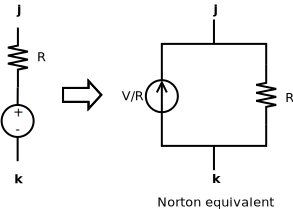
\includegraphics[scale=0.6]{img/RealVoltageSource.png} 
	\caption{Real Voltage Source}
	\label{fig:Real_Voltage_Source}
\end{figure}

The matrix stamp for a real voltage source is therefore as in equation \ref{eq:MatrixStampRealVS}.

\begin{align} \label{eq:MatrixStampRealVS}
\begin{split}
&
\begin{matrix}
& \cdots & j & \quad k & \cdots
\end{matrix}\\[-6pt]
\begin{matrix}
\vdots\\[6pt]
j\\[6pt]
k\\[6pt]
\vdots\\
\end{matrix}
&
\begin{bmatrix}
	\quad & \quad &  \\[6pt]
	\quad & \dfrac{1}{R} & \dfrac{-1}{R} & \quad  \\[6pt]
	\quad & \dfrac{-1}{R} & \dfrac{1}{R} & \quad \\[6pt]
	\quad &  & 
\end{bmatrix}
\begin{bmatrix}
	\quad \\[6pt]
	e_j(k+1)\\[6pt]
	e_k(k+1)\\[6pt]
	\quad
\end{bmatrix}
=
\begin{matrix}
\vdots\\[6pt]
j\\[6pt]
k\\[6pt]
\vdots\\
\end{matrix}
\begin{bmatrix}
	\quad \\[6pt]
	\dfrac{V}{R} \\[6pt]
	-\dfrac{V}{R} \\[6pt]
	\quad
\end{bmatrix}
\end{split}
\end{align}

The following parameters are defined by the user for the real voltage source:

\begin{itemize}
\item name: Name of the component
\item src: Node connected to voltage source positive terminal (j)
\item dest: Node connected to voltage source negative terminal (k)
\item voltage: Voltage in V
\item phase: Phase shift in degrees
\item resistance: Series resistance in ohms 
\end{itemize}

The function "applySystemMatrixStamp" will stamp the resistance at the conductance matrix $G$.
The function "applyRightSideVectorStamp" will stamp the equivalent current source $I=\frac{V}{R}$ to the vector $A$.
The function "step" will repeat the stamp of the vector $A$ each time step.

\subsection{Ideal Voltage Source}

The model of the ideal voltage source uses the modified nodal analysis as presented in subsection \ref{IdealVoltageSource}.
The following parameters are defined by the user:

\begin{itemize}
\item name: Name of the component
\item src: Node connected to voltage source positive terminal
\item dest: Node connected to voltage source negative terminal
\item voltage: Voltage in V
\item phase: Phase shift in degrees
\item num: Number of the voltage source (the voltage sources have to be numbered in sequence) 
\end{itemize}

The function "applyMatrixStamp" will stamp the conductance matrix according to subsection \ref{IdealVoltageSource}. The additional unknown $i_{jk}$ of the voltage source number 1 (with variable num=1) will be added in the first line after the last node voltage and so on. Therefore, for a circuit with n voltage sources and m nodes, the vector of unknown variable $e$ and the vector $A$ will have the size $m+n$. The conductance matrix G will have the size $(m+n)X(m+n)$.

\begin{equation}
	e=
	\begin{bmatrix}
		e_1 \\
		\vdots \\
		e_m \\
		i_1 \\
		\vdots \\
		i_n
	\end{bmatrix}
\end{equation}

The function "applyRightSideVectorStamp" will stamp the voltage at the corresponding line of the vector $A$.
The function step will repeat the stamp of the vector $A$ each time step.

\subsection{Current Source}

For the current source, the following parameters are defined by the user:

\begin{itemize}
\item name: Name of the component
\item src: Node connected to current source positive terminal
\item dest: Node connected to current source negative terminal
\item current: Current in A
\item phase: Phase shift in degrees
\end{itemize}

The function "applyRightSideVectorStamp" will stamp the current at the vector $A$ as in subsection \ref{CurrentSourceMatrixStamp}.